\chapter{均匀物质的热力学性质}
对于非绝热过程,比如恒温恒容过程,可定义Helmholtz自由能
\begin{align}
	F:=U-TS,
\end{align}
Gibbs自由能
\begin{align}
	G:=U-TS+pV,
\end{align}
易证,对于恒温恒容过程$\D F\leqslant 0$;对于恒温恒压过程$\D G\leqslant 0$。
\begin{definition}{特性函数}{characterist funtion}
	适当选取自变量,只需一个热力学量就可决定均匀系统的全部热力学性质,这样的函数称为特性函数(characterist funtion)。
	
	包括$U(S,V),H(T,V),F(S,p),G(T,p)$等。
\end{definition}
\section{Maxwell关系}
由特性函数$U(S,V)$的二阶导
\begin{align}
	\pw USV=\pw UVS,\implies-\kh{\pv pS}_V=\kh{\pv TV}_S;
\end{align}
同理,对$F(T,V),H(S,p),G(T,p)$
\begin{align}
	\pw FTV=\pw FVT,\implies\quad\kh{\pv pT}_V=\kh{\pv SV}_T; \\
	\pw HSp=\pw HpS,\implies\quad\kh{\pv VS}_p=\kh{\pv Tp}_S; \\
	\pw GTp=\pw GpT,\implies-\kh{\pv VT}_p=\kh{\pv Sp}_T.
\end{align}
\begin{center}
	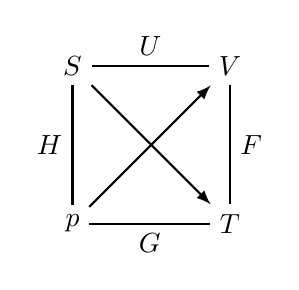
\begin{tikzpicture}
		\node(s)at(0,2){$S$};
		\node(v)at(2,2){$V$};
		\node(p)at(0,0){$p$};
		\node(t)at(2,0){$T$};
		\draw[thick](s)--(v)node[midway,above]{$U$};
		\draw[thick](s)--(p)node[midway,left]{$H$};
		\draw[thick](t)--(v)node[midway,right]{$F$};
		\draw[thick](t)--(p)node[midway,below]{$G$};
		\draw[thick,-latex](s)--(t);
		\draw[thick,-latex](p)--(v);
	\end{tikzpicture}
	\captionof{figure}{Good physicists Have Studied Under Very Fine Teachers.}
\end{center}
熵的标准全微分式:以$p,V,T$中两个为自变量,且将微分前系数用可测量表达出来的全微分式。比如以$T,V$
\[
	\d S=\kh{\pv ST}_V\d T+\kh{\pv SV}_T\d V=\frac{C_V}T\d T+\kh{\pv pT}_V\d V.
\]
\iffalse
\paragraph{附:偏导关系式}
微积分II中我们学过:
\begin{align}
	 & 1.       & \kh{\pv XY}_Z & =\kh{\pv YX}_Z^{-1};                                             \\
	 & 2.       & \kh{\pv XY}_Z & =\dvd{\kh{\pv XW}_Z}{\kh{\pv YW}_Z};  \\
	 & 3.^\star & \kh{\pv XY}_Z & =-\dvd{\kh{\pv ZY}_X}{\kh{\pv ZX}_Y}; \\
	 & 4.       & \kh{\pv XY}_Z & =\kh{\pv XY}_W+\kh{\pv XW}_Y\kh{\pv WY}_Z.
\end{align}
% 可以用Jaccobi行列式证明。
\fi
利用偏导关系式
\begin{align*}
	\kh{\pv ST}_p=\kh{\pv ST}_V+\kh{\pv SV}_T\kh{\pv VT}_p,
\end{align*}
由Maxwell关系
\[
	\kh{\pv SV}_T=\kh{\pv pT}_V=-\dvd{\kh{\pv VT}_p}{\kh{\pv Vp}_T}.
\]
因此
\[
	C_p-C_V=-T\dvd{\kh{\pv VT}_p^2}{\kh{\pv Vp}_T}.
\]

\paragraph{响应函数}定义体膨张系数
\begin{align}
	\alpha:=\frac1V\kh{\pv VT}_p.
\end{align}
等温压缩系数
\begin{align}
	\kappa_T:=-\frac1V\kh{\pv Vp}_T.
\end{align}
可得
\begin{align}
	C_p-C_V=\frac{VT\alpha^2}{\kappa_T}\geqslant 0.
\end{align}